\documentclass[a4paper]{article}
\usepackage[top=1in,bottom=1in,left=1in,right=1in]{geometry}
\usepackage{times}
\usepackage{amssymb}
\usepackage{mathtools}	% pulls in amsmath
	\mathtoolsset{centercolon}
\usepackage{tikz}
	\usetikzlibrary{automata}
	\usepackage{tikz-qtree}
\usepackage{mathpartir}
\usepackage{amsthm}
\usepackage{amsxtra}
\usepackage{algorithm}
\usepackage{algpseudocode}
\usepackage{semantic}
	\reservestyle{\declarevars}{\texttt}
	\reservestyle{\declareops}{\texttt}
	\reservestyle{\declarestates}{\text}
\usepackage{color}
\usepackage{listings}
\usepackage{mathtools}
\usepackage[shortlabels]{enumitem}
\usepackage{graphicx}	% for pdf image

\newtheorem{theorem}{Theorem}

\newtheorem{myexample}{\textbf{Example}}
\newtheorem{mylemma}{\textbf{Lemma}}
\newtheorem{myproof}{\textbf{Proof}}
\newtheorem{myinvariant}{\textbf{Invariant}}
\newtheorem{mytheorem}{\textbf{Theorem}}
\newtheorem{mycorollary}{\textbf{Corollary}}
\newtheorem{myapproach}{Approach}
\newtheorem{myproperty}{Property}
\newtheorem{mydefinition}{Definition}

\newtheorem{mycase}{Case}

\lstset{ %
  backgroundcolor=\color{white},   % choose the background color; you must add \usepackage{color} or \usepackage{xcolor}
  basicstyle=\small,        % the size of the fonts that are used for the code
  breakatwhitespace=false,         % sets if automatic breaks should only happen at whitespace
  breaklines=true,                 % sets automatic line breaking
  captionpos=b,                    % sets the caption-position to bottom
  commentstyle=,    % comment style
  deletekeywords={...},            % if you want to delete keywords from the given language
  escapeinside={\%*}{*)},          % if you want to add LaTeX within your code
  extendedchars=true,              % lets you use non-ASCII characters; for 8-bits encodings only, does not work with UTF-8
 % frame=single,                    % adds a frame around the code
  keepspaces=true,                 % keeps spaces in text, useful for keeping indentation of code (possibly needs columns=flexible)
  columns=fullflexible,	% not monospace
  keywordstyle=,       % keyword style
  language=Octave,                 % the language of the code
  morekeywords={forall, to, else, then, end, and, or, assign, increment, decrement, jump, jump_if, store, *, +},            % if you want to add more keywords to the set
  numbers=left,                    % where to put the line-numbers; possible values are (none, left, right)
  numbersep=5pt,                   % how far the line-numbers are from the code
  rulecolor=\color{black},         % if not set, the frame-color may be changed on line-breaks within not-black text (e.g. comments (green here))
  showspaces=false,                % show spaces everywhere adding particular underscores; it overrides 'showstringspaces'
  showstringspaces=false,          % underline spaces within strings only
  showtabs=false,                  % show tabs within strings adding particular underscores
  stepnumber=1,                    % the step between two line-numbers. If it's 1, each line will be numbered
  stringstyle=,     % string literal style
  tabsize=4,                       % sets default tabsize to 2 spaces
  title=\lstname,                  % show the filename of files included with \lstinputlisting; also try caption instead of title
  mathescape,
  belowskip=-\baselineskip,
}

\DeclareMathOperator{\prob}{prob}
\DeclareMathOperator{\dom}{dom}
\DeclareMathOperator{\rank}{rank}
\DeclareMathOperator{\key}{key}
\newcommand*{\floor}[1]{\left\lfloor{#1}\right\rfloor}
\newcommand*{\ceil}[1]{\left\lceil{#1}\right\rceil}
\newcommand{\any}{{\rule[-.2ex]{1ex}{.4pt}}}	% Less hideous than \_.
\newcommand{\RR}{\mathbb{R}}
\newcommand{\NN}{\mathbb{N}}
\newcommand{\ZZ}{\mathbb{Z}}
\newcommand{\RP}{\RR_{\ge 0}}
\newcommand*{\dave}[1]{{\color{red}\textbf{PDS: #1}}}
\newcommand{\ie}{\emph{i.e.,} }
\newcommand{\eg}{\emph{e.g.,} }
\usepackage{hyperref}
\newcommand*{\Sref}[1]{\hyperref[#1]{\S\ref*{#1}}}
\newcommand*{\figref}[1]{\hyperref[#1]{Figure~\ref*{#1}}}
\newcommand{\edge}{\longrightarrow}
\newcommand{\redge}{\longleftarrow}

\title{Exercise Sheet 6---Algorithms and Data Structures}
\author{Felipe Cerqueira \\ 2547787 \and David Swasey \\ 2542105}

\begin{document}

\maketitle

Tutorial time: Monday 14:00

\section*{Exercise 1 (15 pts)}

Let $G$ be a directed graph, where each edge is colored either red or blue.
Let $u$ and $v$ be two vertices of $G$.
\begin{enumerate}[a)]
	\item Design an efficient algorithm to decide whether there exists a directed path from $u$ to $v$ that contains at least twice as many red edges as blue edges.
	
	\item Design an efficient algorithm for finding a path from $u$ to $v$ that contains as few red edges as possible.
	
	\item Design an efficient algorithm for finding a path from $u$ to $v$ that contains exactly two red edges, if such a path exists, or otherwise reports failure.
\end{enumerate}

\paragraph{Answer for (1a).}
We proceed as follows.
\begin{itemize}
	\item
	Modify Bellman-Ford to mark every node $w$ s.t.\ there exists a negative cycle involving $w$.
	
	\item
	Run this algorithm with start node $u$ and cost function $c(e) = -1$ if $e$ red; $2$ otherwise.
	
	\item
	If it reports no negative cycles, then (i)~output YES if $d[v] \le 0$, otherwise NO and (ii)~halt.
	
	\item
	Let  $m : V \to \{0,1\}$ be the marks.
	
	Observe that for every $w$ s.t.\ $m[w] = 1$, there exists a red cycle in $G$ reachable from $u$.
	Thus if we can reach $v$ from any such $w$, then we can output YES: Let $p$ be a path from $u$ to $v$ that touches such a cycle, $C$, at some marked vertex $w$.
	Let $k$ be the number of blue edges on $p$.
	Extend $p$ at $w$ by going round the cycle $2k$ times.
	Output YES.

	\item
	Run DFS on $G^\text{op}$ (edges reversed) from $v$, searching for such a $w$ and treating it as indicated.

\end{itemize}

\paragraph{Answer for (1b).}
We use Dijkstra's algorithm to solve this in $O(E + V \log V)$ time.
	Define $c(e) := 1$ if $e$ red; $0$ otherwise.
	Run Dijkstra's algorithm with source $u$.
	Return the shortest path to $v$, if any.

\paragraph{Answer for (1c).}
We represent sets of vertices $S \subseteq V$ using bit vectors or by reserving bits in each vertex.
This makes initialization ($S \gets \emptyset$) linear, update ($S \gets S \cup \{ x \}$) constant, and intersection ($S \cap S'$) linear.
We omit the details.

Assume a function search$(G, x)$ that runs in time $O(V+E)$ and returns the set of vertices reachable from $x$ by paths containing exactly one red edge.
Given such a function, we proceed as follows.
\begin{itemize}
	\item
	$O(V+E)$: $S_1 \gets \text{search}(G, u)$

	\item
	$O(V+E)$: $S_2 \gets \text{search}(G^\text{op}, v)$, where $G^\text{op}$ has edges reversed

	\item
	$O(V):$ Output YES if $S_1 \cap S_2 \not= \emptyset$; otherwise NO.
\end{itemize}
The search function is implicitly parameterized by a graph $G=(V,E)$.
It's a simple variant on DFS and uses an additional set $M$ of marked nodes:
\begin{lstlisting}[numbers=none,xleftmargin=1cm]
search$(s)$:
	$S \gets \emptyset$; $M \gets \emptyset$
	dfs$(s, 0)$
	return $S$
save$(x, b)$: if $b=1$ then $S \gets S \cup \{ x \}$
dfs$(x, b)$:
	save$(x, b)$
	$M \gets M \cup \{ x \}$
	for $y \in \text{Adj}[x]$
		if $b=1 \land (x,y)$ red
			continue
		$b' \gets$ if $(x,y)$ red then $1$ else $0$
		if $y \in M$ then save$(y, b')$ else dfs$(y, b')$\end{lstlisting}
The search proceeds in two stages.
When $b=0$, red edges cause us to flip $b$.
When $b=1$, we save visited vertices (as well as vertices reachable by back and cross edges) in $S$ and we avoid traversing red edges.

\section*{Exercise 2 (5 pts)}

Show that Dijkstra's algorithm can fail on graphs with negative costs.

\paragraph{Answer:}
On removing a node $v$ from its queue, Dijkstra's algorithm assumes that its estimate for $v$ is tight (\ie $d[v] = \mu(s, v)$) and that, if $\pi[v] \not= \bot$, then the parent pointers $\pi$ lead to $s$ and describe a path from $s$ to $v$ with this minimal cost.
If the queue contains some node $w$ such that an edge $(w, v)$ exists, then, \emph{assuming non-negative edge costs,} we know that we cannot use $w$ to construct a better path for $v$.
The invariant---that we're ``finished'' with $v$ once we remove it from the queue---breaks down with negative edge costs.
After removing $v$ from the queue, we may later find a node $w$ such that the path through $w$ lowers the cost of reaching $v$.
We weren't ``finished'' with $v$, after all.

\begin{figure}
\centering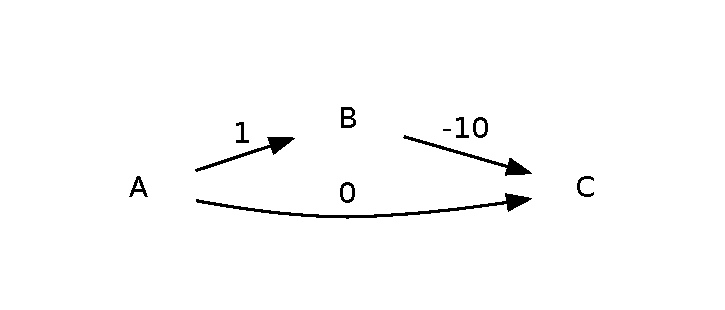
\includegraphics{ex07ex2.pdf}
\caption{Counterexample for Dijkstra with negative weights.}
\label{fig:dijkstraeg}
\end{figure}

It's easy to give a counterexample, once we fix the code.
We prefer to build the heap up-front, and to only relax edges to nodes that are not in the heap:
\begin{lstlisting}[numbers=none,xleftmargin=1cm]
dijkstra$(s)$:
	$\pi \gets \text{array}(|V|, \bot)$; $d \gets \text{array}(|V|, \infty)$; $d[s] \gets 0$
	$Q \gets \text{makeheap}(V)$	; priorities $d[v]$
	while $Q \not= \emptyset$
		let $v = \text{deleteMin}(Q)$
		for every $w$ s.t. $v \edge w$	; adj. list
			if $w \in Q$ then
				relax$(v, w)$	% adjusts priority in $Q$
\end{lstlisting}
We omit the evident code for relax.
(Note that the test $w \in Q$ can be implemented in $O(1)$ time and space using mark bits in nodes.
After makeheap, we mark every node as in $Q$.
When deleteMin returns $v$, we clear $v$'s mark.)
Now consider what happens when we run this code on the graph in \figref{fig:dijkstraeg} with source $A$.
We dequeue the nodes in order $A$, $C$, and $B$.
After initialization, $d = \{ A \mapsto 0; C, B \mapsto \infty \}$ and we dequeue $A$.
After relaxing from $A$, we have the ``shortest path forest'' (\ie $\pi$ and $d$)
\[
	\Tree [.$0A$ $0C$ $1B$ ]
\]
Thereafter, the forest never changes.
On termination, the forest says that the shortest path from $A$ to $C$ has zero cost and comprises the edge $A \edge C$.
That's wrong.
The shortest path  $A \edge B \edge C$ has cost $-9$.

\section*{Exercise 3 (15 pts)}

Consider the following algorithm for solving the single-source shortest path problem in directed graphs with general edge costs:

\begin{lstlisting}[mathescape]
SSSP(V ,E,c,s):
    Improved = {s}
    while Improved $\neq \emptyset$ do
        B = Improved
        Improved = $\emptyset$
        while B $\neq \emptyset$
            choose and remove some v from B
            for each w in Out(v) do
                d’ = d[v] + c((v,w))
                if d’ < d[w] then
                    d[w] = d’
                    parent[w] = v
                    insert w into Improved
\end{lstlisting}

Assume Out(v) denotes the set of out-neighbors of v, and sets B and Improved are implemented such that insertions, deletions, choosing some element, and test for emptiness only need constant time each.

\paragraph{a)} Does this program always terminate? If no, correct it appropriately.

\paragraph{Answer:}

No, it doesn't terminate if there are negative cycles. When there is a negative cycle between two nodes, the shortest path keeps improving. We can fix the algorithm by limiting the number of improvements to $n-1$:

\begin{lstlisting}[mathescape, commentstyle=\color{red}, keywordstyle=\color{blue}]
SSSP(V,E,c,s):
    foreach $v \in V$ do
        count[v] = 0 % number of improvements
    Improved = {s}
    while Improved $\neq \emptyset$ do
        B = Improved
        Improved = $\emptyset$
        while B $\neq \emptyset$
            choose $\text{and}$ remove some v from B
            foreach w in Out(v) do
                d’ = d[v] + c((v,w))
                if d’ < d[w] then
                    if count[w] < $n-1$ % Limit number of improvements for an edge
                        d[w] = d’
                        parent[w] = v
                        insert w into Improved
                        count[w] = count[w] + 1
                    else
                        d[w] = $-\infty$
\end{lstlisting}


\paragraph{b)} Show that there are arbitrarily large graphs for which SSSP() is asymptotically faster than the Bellman-Ford algorithm

\paragraph{Answer:}

The Bellman-Ford algorithm will invariably relax all the edges $(n-1)$ times, but SSSP() will perform much better in graphs with faster convergence, like this star graph. Here, each edge will not improve anymore after the first relaxation.

\begin{center}
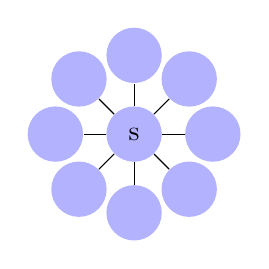
\begin{tikzpicture}[main_node/.style={circle,fill=blue!30,minimum size=2em,inner sep=3pt]}]

    \node[main_node] (1) at (0,0) {s};
    \node[main_node] (2) at (-1, 0)  {};
    \node[main_node] (3) at (1, 0) {};
    \node[main_node] (4) at (0, 1) {};
    \node[main_node] (5) at (0, -1) {};
    \node[main_node] (6) at (0.7, 0.7) {};
    \node[main_node] (7) at (-0.7, -0.7) {};
    \node[main_node] (8) at (0.7, -0.7) {};
    \node[main_node] (9) at (-0.7, 0.7) {};
    \draw (1) -- (2);
    \draw (1) -- (3);
    \draw (1) -- (4);
    \draw (1) -- (5);
    \draw (1) -- (6);
    \draw (1) -- (7);
    \draw (1) -- (8);
    \draw (1) -- (9);
\end{tikzpicture}
\end{center}


\paragraph{c)} Show that there are arbitrarily large graphs for which SSSP() has the same asymptotic running time as the Bellman-Ford algorithm.

\paragraph{Answer:}

SSSP() will have the same asymptotic running time as Bellman-Ford in graphs that require $(n-1)$ relaxation rounds for all edges, in order to detect negative cycles.
Here, the path from $S$ to every node will be improved $(n-1)$ times until all distances become $-\infty$.

\begin{center}
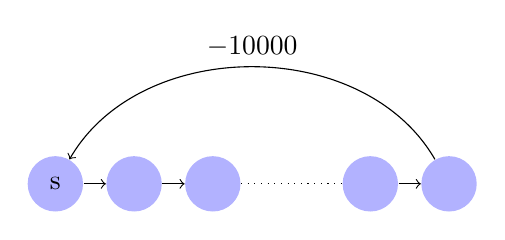
\begin{tikzpicture}[main_node/.style={circle,fill=blue!30,minimum size=2em,inner sep=3pt]}]

    \node[main_node] (1) at (0,0) {s};
    \node[main_node] (2) at (1, 0)  {};
    \node[main_node] (3) at (2, 0) {};
    \node[main_node] (4) at (4, 0) {};
    \node[main_node] (5) at (5, 0) {};
    \begin{scope}[every path/.style={->}]
    \draw (1) -- (2);
    \draw (2) -- (3);
    \draw (4) -- (5);
    \end{scope}
    \begin{scope}[every path/.style={dotted}]
       \draw (3) -- (4);
    \end{scope}

\begin{scope}[every path/.style={->}]    
    %\path (2) edge [bend left=60] node [below] {$-1$} (1);
    %\path (3) edge [bend right=60] node [above] {$-1$} (1);
    %\path (4) edge [bend left=60] node [below] {$-1$} (1);
    \path (5) edge [bend right=60] node [above] {$-10000$} (1);      
\end{scope}
\end{tikzpicture}
\end{center}

\section*{Exercise 4 (15 pts)}

Due to recent strikes in German railway companies, Saarstahl is considering to increase the use of trucks for transportation. They want to send trucks from Völklingen to Rotterdam harbor laden as heavily as possible with steel products, but each road segment has a maximum weight limit on trucks that use this road.

\paragraph{a)} Give an efficient algorithm for finding a route that allows to load a truck with maximum possible weight.

\paragraph{Answer:} We can represent the problem with a graph where the vertices represent the cities, and each edge $e$ represents a road segment of maximum weight limit $w(e)$. To solve the problem, we associate to each edge a cost $-w(e)$, and then we can apply the shortest path algorithm starting from Volklingen to find the best path that leads to Rotterdam.

\paragraph{b)} An ordered semigroup is a set S together with an operation $\oplus$, a neutral element 0, and a linear ordering $\le$ such that for all $x, y, z \in S$ we have
\begin{itemize}
\item $x \oplus y \in S$,
\item $(x \oplus y)=(y \oplus x)$,
\item $(x \oplus y) \oplus z=x \oplus (y \oplus z)$,
\item $x \oplus 0=x$, and
\item $x \le y \implies x \oplus z \le y \oplus z$.
\end{itemize}

Show how the Bellman-Ford algorithm can be applied when edge weights in a graph come from an ordered semigroup.

\paragraph{Answer:}

We can just pretend this ordered semigroup are the integer numbers we are already used to. Whenever we use the integer $0$, we replace it with the neutral element of the group. And whenever we use $+$ (addition) and $\le$ (less-than-or-equal-to), we replace them with $\oplus$ and the order $\le$ from the group, respectively. Also, the absence of an edge can be represented by a large dummy cost (with respect to $\le$).

\paragraph{c)} Under which conditions can Dijkstra’s algorithm be applied when edge weights in a graph come from an ordered semigroup? Under which conditions can we use the APSP algorithm from the lecture?

\paragraph{Answer:}

To apply Dijkstra's algorithm, we need to guarantee the absence of negative edges, with an extra constraint $0 \le x$.

To use the APSP algorithm from the lecture, we need to guarantee non-negative cycles.
I think there is no way to encode this property by restricting the set of possible edge costs, since this does not capture reachability in the graph. But we can definitely be conservative and prevent negative cycles by also forcing $0 \le x$.
\end{document}